\documentclass[12pt]{article}
\usepackage[utf8]{inputenc}
\usepackage{amsmath}
\usepackage{amssymb}
\usepackage{geometry}
\usepackage{listings}
\usepackage{xcolor}
\usepackage{hyperref}
\usepackage{booktabs}
\usepackage{array}
\usepackage{graphicx}
\usepackage{float}
\usepackage{enumitem}
\usepackage{tikz}
\usetikzlibrary{matrix,positioning}

\geometry{a4paper, margin=1in}

\definecolor{codegreen}{rgb}{0,0.6,0}
\definecolor{codegray}{rgb}{0.5,0.5,0.5}
\definecolor{codepurple}{rgb}{0.58,0,0.82}
\definecolor{backcolour}{rgb}{0.95,0.95,0.92}

\lstset{
    backgroundcolor=\color{backcolour},
    commentstyle=\color{codegreen},
    keywordstyle=\color{magenta},
    numberstyle=\tiny\color{codegray},
    stringstyle=\color{codepurple},
    basicstyle=\ttfamily\small,
    breakatwhitespace=false,
    breaklines=true,
    captionpos=b,
    keepspaces=true,
    numbers=left,
    numbersep=5pt,
    showspaces=false,
    showstringspaces=false,
    showtabs=false,
    tabsize=2,
    language=Python
}

\title{%
    \large 8th Semester Artificial Intelligence Laboratory 2026 \\[4pt]
    \large CS 4271 \\[10pt]
    \textbf{\LARGE ASSIGNMENT -- 5} \\[8pt]
    \textbf{\Large Connect-4 Game} \\[4pt]
    \large Mini-Max Algorithm with Alpha-Beta Pruning
}
\author{Uttam Mahata (2022CSB104)}
\date{\today}

\begin{document}

\maketitle
\tableofcontents
\newpage

% -----------------------------------------------------------------------------
\section{Introduction}
% -----------------------------------------------------------------------------

Connect-4 is a classic two-player strategy game played on a
\textbf{6-row $\times$ 7-column} vertical grid.
Players alternate dropping coloured discs into columns; each disc falls under
gravity to the lowest available row in that column.
The first player to form a line of \textbf{four consecutive discs}
(horizontally, vertically, or diagonally) wins.

This implementation pits a \textbf{human player} against a
\textbf{computer AI} that uses the \textbf{Mini-Max algorithm with
alpha-beta pruning} to determine the optimal move at every turn.

Key features of this implementation:
\begin{itemize}
    \item Full 6$\times$7 Connect-4 game with gravity-based disc placement.
    \item Mini-Max search to depth 5 with alpha-beta pruning for efficiency.
    \item Heuristic evaluation function encoding three winning strategies
          (centre preference, opponent blocking, multi-directional threats).
    \item Interactive console interface with ASCII board visualisation.
    \item Dual output: terminal display and \texttt{output.txt} game log.
\end{itemize}

% -----------------------------------------------------------------------------
\section{Problem Formulation}
% -----------------------------------------------------------------------------

\subsection{State Space}

A game state is a complete snapshot of the board at any point in time.
Formally:
\[
    \mathcal{S} = \{0, 1, 2\}^{6 \times 7}
\]
where each cell value is:
\begin{itemize}
    \item \texttt{0} (EMPTY) --- no disc placed.
    \item \texttt{1} (PLAYER) --- human disc (\textbf{O}).
    \item \texttt{2} (AI) --- computer disc (\textbf{X}).
\end{itemize}

The board is stored as a 2-D NumPy array of shape $(6, 7)$.
Row~0 is the \emph{top}; row~5 is the \emph{bottom}.
Gravity is simulated by always inserting a disc into the lowest empty row of
the chosen column.

\subsection{Actions}

At any turn, the set of legal actions is:
\[
    \mathcal{A}(s) = \{ c \in \{0,\ldots,6\} \mid s[0][c] = \texttt{EMPTY} \}
\]
i.e.\ all columns that still have at least one empty cell.

\subsection{Terminal States}

A state $s$ is terminal if any of the following hold:
\begin{enumerate}
    \item The AI has four discs in a row (AI wins).
    \item The human has four discs in a row (human wins).
    \item All 42 cells are occupied (draw).
\end{enumerate}

\subsection{Win Condition}

Four consecutive discs of the same player in any of the following directions
constitutes a win:

\begin{center}
\begin{tabular}{@{} l l @{}}
\toprule
\textbf{Direction} & \textbf{Window pattern} \\
\midrule
Horizontal  & $(r,c),\,(r,c{+}1),\,(r,c{+}2),\,(r,c{+}3)$ \\
Vertical    & $(r,c),\,(r{+}1,c),\,(r{+}2,c),\,(r{+}3,c)$ \\
Diagonal~$\nearrow$ & $(r,c),\,(r{+}1,c{+}1),\,(r{+}2,c{+}2),\,(r{+}3,c{+}3)$ \\
Diagonal~$\searrow$ & $(r,c),\,(r{-}1,c{+}1),\,(r{-}2,c{+}2),\,(r{-}3,c{+}3)$ \\
\bottomrule
\end{tabular}
\end{center}

% -----------------------------------------------------------------------------
\section{Winning Strategies}
% -----------------------------------------------------------------------------

Three strategies from the assignment specification are encoded directly into
the AI's heuristic function.

\subsection{Strategy (a): Middle Column Placement}

The centre column (column~3) provides the maximum number of potential
four-in-a-row connections --- up to five different winning lines pass through
it.  The heuristic awards \textbf{+3 points} for every AI disc in column~3:

\begin{lstlisting}[caption={Centre column bonus in score\_position.}]
center_col = list(board[:, COLS // 2])   # column 3
score += center_col.count(piece) * 3
\end{lstlisting}

This causes the AI to prefer column~3 on the opening move.

\subsection{Strategy (b): Trapping / Blocking Opponents}

A window containing \emph{three opponent discs and one empty cell} is an
immediate threat.  The heuristic applies a \textbf{$-4$ penalty} to such
windows, forcing the AI to prioritise blocking:

\begin{lstlisting}[caption={Opponent threat penalty in score\_window.}]
elif opp_count == 3 and empty == 1:
    return -4
\end{lstlisting}

When the AI encounters a board where the human has three in a row, the
negative score dominates and the AI's best response is to drop into the
blocking cell.

\subsection{Strategy (c): ``7'' Formation (Multi-directional Threats)}

By evaluating \emph{all} windows (horizontal, vertical, both diagonals)
simultaneously and searching to depth~5, the Mini-Max tree naturally
discovers positions where the AI threatens to win in multiple directions at
once --- equivalent to the ``7'' formation described in the assignment.
No single window can be blocked without the opponent winning via another.

% -----------------------------------------------------------------------------
\section{Mini-Max Algorithm}
% -----------------------------------------------------------------------------

\subsection{Overview}

Mini-Max is a recursive \emph{backtracking} algorithm for two-player
zero-sum games.  It models:
\begin{itemize}
    \item The \textbf{maximising player} (AI) --- tries to reach states with
          the highest heuristic score.
    \item The \textbf{minimising player} (human) --- tries to reach states
          with the lowest heuristic score.
\end{itemize}

Both players are assumed to play \emph{optimally}.

\subsection{Evaluation Function}

The heuristic $h(s)$ scores a board state $s$ from the AI's perspective.
It examines every \emph{window} of 4 consecutive cells across all directions:

\begin{equation}
h(s) = \underbrace{3 \cdot |\text{AI discs in col 3}|}_{\text{centre bonus}}
     + \sum_{\text{windows } w} \textit{scoreWindow}(w, \text{AI})
\end{equation}

\textbf{Window scoring} (\texttt{score\_window}):

\begin{table}[H]
\centering
\begin{tabular}{@{} l c @{}}
\toprule
\textbf{Window contents} & \textbf{Score} \\
\midrule
4 AI discs                         & $+100$ \\
3 AI discs $+$ 1 empty             & $+5$   \\
2 AI discs $+$ 2 empty             & $+2$   \\
3 opponent discs $+$ 1 empty       & $-4$   \\
All other configurations           & $0$    \\
\bottomrule
\end{tabular}
\caption{Heuristic window scores.}
\end{table}

\subsection{Recursive Definition}

Let $d$ be the remaining search depth.  The Mini-Max value is:

\begin{equation}
\text{minimax}(s, d, \alpha, \beta, \textit{max}) =
\begin{cases}
+10^8 & \text{if AI wins in } s \\
-10^8 & \text{if human wins in } s \\
h(s)  & \text{if } d = 0 \text{ or board full} \\[4pt]
\displaystyle\max_{a \in \mathcal{A}(s)}\;\text{minimax}(s_a, d{-}1, \alpha, \beta, \texttt{False})
       & \text{if } \textit{max} = \texttt{True} \\[6pt]
\displaystyle\min_{a \in \mathcal{A}(s)}\;\text{minimax}(s_a, d{-}1, \alpha, \beta, \texttt{True})
       & \text{if } \textit{max} = \texttt{False}
\end{cases}
\end{equation}

where $s_a$ is the board state after action $a$ is applied.

\subsection{Algorithm Pseudocode}

\begin{lstlisting}[language={}, caption={Mini-Max with Alpha-Beta Pruning (pseudocode)}, mathescape=true]
Input:  board s, depth d, alpha $\alpha$, beta $\beta$, maximising flag
Output: (best_column, score)

minimax(s, d, $\alpha$, $\beta$, maximising):
    if AI wins(s):     return (None, +1e8)
    if human wins(s):  return (None, -1e8)
    if d=0 or full(s): return (None, h(s))

    valid <- { c | s[0][c] = EMPTY }

    if maximising:
        value    <- -inf
        best_col <- random(valid)
        for c in valid:
            drop AI disc in column c -> s'
            _, score <- minimax(s', d-1, $\alpha$, $\beta$, False)
            if score > value:
                value <- score ;  best_col <- c
            $\alpha$ <- max($\alpha$, value)
            if $\alpha$ >= $\beta$: break      -- $\beta$ cut-off

    else:
        value    <- +inf
        best_col <- random(valid)
        for c in valid:
            drop human disc in column c -> s'
            _, score <- minimax(s', d-1, $\alpha$, $\beta$, True)
            if score < value:
                value <- score ;  best_col <- c
            $\beta$ <- min($\beta$, value)
            if $\alpha$ >= $\beta$: break      -- $\alpha$ cut-off

    return (best_col, value)
\end{lstlisting}

% -----------------------------------------------------------------------------
\section{Alpha-Beta Pruning}
% -----------------------------------------------------------------------------

\subsection{Motivation}

Pure Mini-Max with branching factor $b = 7$ and depth $d = 5$ visits up to
$b^d = 7^5 = 16\,807$ leaf nodes per move.  Alpha-beta pruning eliminates
subtrees that cannot affect the final decision, reducing this in practice to
$O(b^{d/2})$ --- equivalent to doubling the effective search depth.

\subsection{Cut-off Conditions}

Two variables are maintained throughout the recursive search:

\begin{itemize}
    \item $\alpha$ --- the \emph{best score the maximiser can guarantee} so
          far on the path from the root.  Initialised to $-\infty$.
    \item $\beta$  --- the \emph{best score the minimiser can guarantee} so
          far on the path from the root.  Initialised to $+\infty$.
\end{itemize}

\textbf{Beta cut-off} (maximising node): if the current value $v \geq \beta$,
the minimiser will never allow this branch --- prune remaining siblings.

\begin{equation}
\alpha \gets \max(\alpha,\, v) \qquad
\text{prune if } \alpha \geq \beta
\end{equation}

\textbf{Alpha cut-off} (minimising node): if the current value $v \leq \alpha$,
the maximiser will never follow this branch --- prune remaining siblings.

\begin{equation}
\beta \gets \min(\beta,\, v) \qquad
\text{prune if } \alpha \geq \beta
\end{equation}

\subsection{Example Cut-off}

\begin{center}
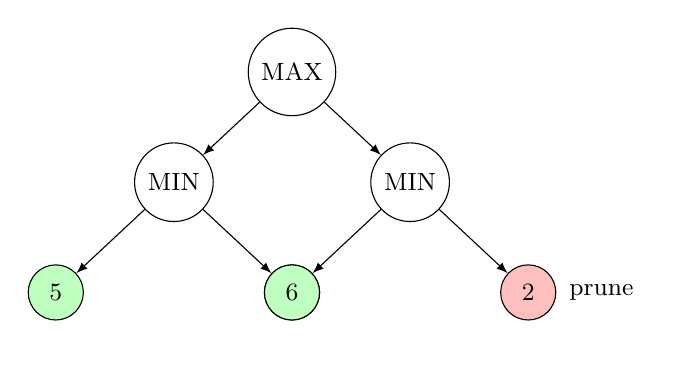
\begin{tikzpicture}[
    level distance=1.4cm,
    sibling distance=3cm,
    every node/.style={draw, circle, minimum size=7mm, font=\small},
    edge from parent/.style={draw,-latex}
]
\node (root) {MAX}
  child { node {MIN}
      child { node[fill=green!25] {5} }
      child { node[fill=green!25] {3} }
  }
  child { node {MIN}
      child { node[fill=green!25] {6} }
      child { node[fill=red!25, label=right:{\small prune}] {2} }
  };
\end{tikzpicture}
\end{center}

After the left MIN-node returns 3, $\alpha = 3$.  In the right MIN-node,
after seeing child value 2, $\beta = 2 \leq \alpha = 3$, so the remaining
children are pruned.

% -----------------------------------------------------------------------------
\section{Implementation}
% -----------------------------------------------------------------------------

\subsection{Module Structure}

\begin{lstlisting}[caption={Module-level layout of connect4.py}]
connect4.py
|- Constants  (ROWS, COLS, EMPTY, PLAYER, AI, DEPTH)
|- Connect4                         # game + AI encapsulated in one class
|   |- __init__()                  # initialise 6x7 numpy board
|   |- tee(*args)                  # print and log simultaneously
|   |- is_valid_column(col)        # True if column has space
|   |- get_next_open_row(col)      # lowest empty row (on self.board)
|   |- drop_piece(board,row,col,p) # place disc in-place
|   |- is_board_full()             # check draw condition
|   |- winning_move(board, piece)  # 4-in-a-row detection
|   |- score_window(window, piece) # heuristic for one window of 4
|   |- score_position(board,piece) # full board heuristic
|   |- minimax(board,d,a,b,max)    # Mini-Max with alpha-beta
|   |- _get_open_row(board, col)   # helper (works on any board copy)
|   |- get_best_move()             # calls minimax, returns best column
|   |- print_board()               # ASCII visualisation
|   |- play()                      # main interactive game loop
|- __main__                        # entry point
\end{lstlisting}

\subsection{Board Representation}

\begin{lstlisting}[caption={Board initialisation.}]
self.board = np.zeros((ROWS, COLS), dtype=int)
# ROWS=6, COLS=7
# board[0][c] = top row  (gravity fills from bottom up)
# board[5][c] = bottom row
\end{lstlisting}

\subsection{Win Detection}

\begin{lstlisting}[caption={winning\_move --- horizontal check shown as example.}]
def winning_move(self, board, piece):
    # Horizontal
    for r in range(ROWS):
        for c in range(COLS - 3):
            if all(board[r][c + i] == piece for i in range(4)):
                return True
    # (vertical, diagonal-positive, diagonal-negative omitted for brevity)
    return False
\end{lstlisting}

\subsection{Heuristic Evaluation}

\begin{lstlisting}[caption={score\_position --- full board evaluation.}]
def score_position(self, board, piece):
    score = 0
    # Strategy (a): centre column bonus
    center_col = list(board[:, COLS // 2])
    score += center_col.count(piece) * 3

    # Horizontal windows
    for r in range(ROWS):
        row_arr = list(board[r, :])
        for c in range(COLS - 3):
            score += self.score_window(row_arr[c:c + 4], piece)

    # Vertical windows
    for c in range(COLS):
        col_arr = list(board[:, c])
        for r in range(ROWS - 3):
            score += self.score_window(col_arr[r:r + 4], piece)

    # Diagonal (positive and negative slopes)
    for r in range(ROWS - 3):
        for c in range(COLS - 3):
            window = [board[r + i][c + i] for i in range(4)]
            score += self.score_window(window, piece)
    for r in range(3, ROWS):
        for c in range(COLS - 3):
            window = [board[r - i][c + i] for i in range(4)]
            score += self.score_window(window, piece)
    return score
\end{lstlisting}

\subsection{Core Mini-Max (Maximising Branch)}

\begin{lstlisting}[caption={Mini-Max maximising branch with beta cut-off.}]
if maximizing_player:
    value    = -math.inf
    best_col = random.choice(valid_cols)

    for col in valid_cols:
        row    = self._get_open_row(board, col)
        b_copy = board.copy()
        b_copy[row][col] = AI

        _, new_score = self.minimax(b_copy, depth - 1,
                                    alpha, beta, False)
        if new_score > value:
            value    = new_score
            best_col = col

        alpha = max(alpha, value)
        if alpha >= beta:          # beta cut-off
            break

    return best_col, value
\end{lstlisting}

% -----------------------------------------------------------------------------
\section{Example Game State}
% -----------------------------------------------------------------------------

\subsection{Board Notation}

During a game session the board is rendered as:

\begin{center}
\begin{verbatim}
+---+---+---+---+---+---+---+
| . | . | . | . | . | . | . |
+---+---+---+---+---+---+---+
| . | . | . | . | . | . | . |
+---+---+---+---+---+---+---+
| . | . | . | X | . | . | . |
+---+---+---+---+---+---+---+
| . | . | . | X | . | . | . |
+---+---+---+---+---+---+---+
| . | . | . | X | O | . | . |
+---+---+---+---+---+---+---+
| . | . | . | O | O | O | . |
+---+---+---+---+---+---+---+
 0   1   2   3   4   5   6
\end{verbatim}
\end{center}

\subsection{Heuristic Trace}

For the board above, the AI (X) evaluates the position:

\begin{itemize}
    \item Column~3 centre bonus: 3 discs $\times$ 3 = \textbf{+9}.
    \item Vertical window \{X,X,X,\texttt{.}\} in column~3 rows 2--5:
          3 AI + 1 empty $\Rightarrow$ \textbf{+5}.
    \item Human window \{O,O,O,\texttt{.}\} in row~5 cols 3--6:
          3 opp + 1 empty $\Rightarrow$ \textbf{-4}.
\end{itemize}

The blocking penalty ($-4$) signals the AI to drop into column~6
(or whichever cell completes the block) before extending its own vertical
threat --- this is Strategy~(b) in action.

% -----------------------------------------------------------------------------
\section{Complexity Analysis}
% -----------------------------------------------------------------------------

\begin{table}[H]
\centering
\begin{tabular}{@{} l l l @{}}
\toprule
\textbf{Component} & \textbf{Time} & \textbf{Space} \\
\midrule
Naive Mini-Max (depth $d$, branching $b$)  & $O(b^d)$        & $O(bd)$ \\
With alpha-beta pruning (best case)        & $O(b^{d/2})$    & $O(bd)$ \\
With alpha-beta pruning (average case)     & $O(b^{3d/4})$   & $O(bd)$ \\
\texttt{score\_position} per call          & $O(R \cdot C)$  & $O(1)$  \\
\texttt{winning\_move} per call            & $O(R \cdot C)$  & $O(1)$  \\
\midrule
\textbf{Per-move total} ($b=7$, $d=5$)    & $\approx$1,000 -- 5,000 nodes & $O(35)$ \\
\bottomrule
\end{tabular}
\caption{Asymptotic complexity ($R=6$ rows, $C=7$ cols, $b=7$, $d=5$).}
\end{table}

Alpha-beta pruning effectively reduces the search tree from $7^5 = 16\,807$
nodes to roughly $7^{2.5} \approx 1{,}297$ nodes in the best case, enabling
depth-5 search to complete in well under a second per move.

% -----------------------------------------------------------------------------
\section{Edge Cases}
% -----------------------------------------------------------------------------

\begin{enumerate}
    \item \textbf{Full column input:}
          The game loop re-prompts the human with an error message rather
          than accepting an invalid column.
    \item \textbf{Non-integer input:}
          A \texttt{ValueError} is caught and the player is asked again.
    \item \textbf{Out-of-range column:}
          Columns outside $[0, 6]$ are rejected before any board access.
    \item \textbf{Draw (board full, no winner):}
          Detected after every move via \texttt{is\_board\_full()}.
    \item \textbf{Depth-0 leaf with no terminal:}
          \texttt{score\_position} is called to return a heuristic value
          without requiring a terminal state.
    \item \textbf{Only one valid column remaining:}
          Mini-Max still evaluates it correctly; alpha-beta pruning simply
          has nothing to prune.
\end{enumerate}

% -----------------------------------------------------------------------------
\section{Usage}
% -----------------------------------------------------------------------------

\begin{lstlisting}[language=bash, caption={Running the game.}]
# Activate virtual environment (if using uv)
source .venv/bin/activate

# Run from the project root
python Assignment-5/connect4.py
\end{lstlisting}

\begin{center}
\begin{tabular}{@{} l l @{}}
\toprule
\textbf{Symbol} & \textbf{Meaning} \\
\midrule
\texttt{.} & Empty cell \\
\texttt{O} & Human disc \\
\texttt{X} & Computer (AI) disc \\
\bottomrule
\end{tabular}
\end{center}

Enter a column number (0--6) when prompted.  The AI responds immediately.
A full game log is saved to \texttt{output.txt} in the current working
directory after the session ends.

% -----------------------------------------------------------------------------
\section{Conclusion}
% -----------------------------------------------------------------------------

This implementation demonstrates the Mini-Max algorithm as an effective AI
for Connect-4.  Key design decisions:

\begin{itemize}
    \item \textbf{Alpha-beta pruning} --- eliminates provably irrelevant
          subtrees, enabling depth-5 search with negligible latency.
    \item \textbf{Centre-column heuristic} --- encodes domain knowledge that
          column~3 is the strategically strongest opening position.
    \item \textbf{Window-based evaluation} --- the same \texttt{score\_window}
          function uniformly handles all four directions, keeping the
          heuristic concise and consistent.
    \item \textbf{Threat-blocking penalty} --- a $-4$ score for opponent
          three-in-a-row windows guarantees the AI blocks immediate threats
          before pursuing its own longer-term plans.
    \item \textbf{Configurable depth} --- the \texttt{DEPTH} constant can be
          increased for stronger (slower) play or decreased for faster
          (weaker) play without any other code changes.
\end{itemize}

\end{document}
